	% 封面（蓝色系）
\begin{titlepage}
	\thispagestyle{empty}
	\begin{tikzpicture}[remember picture,overlay]
		\fill[LogicBlue!85]
		(current page.south west) rectangle
		([xshift=2.8cm]current page.north west);
		\draw[LogicDarkBlue,line width=1pt]
		([xshift=2.8cm]current page.south west) --
		([xshift=2.8cm]current page.north west);
	\end{tikzpicture}
	\vspace*{2cm}
	\hspace*{3.3cm}
	\begin{minipage}{0.7\textwidth}
		
		{\Huge\bfseries 逻辑学基础\par}
		\vspace{0.6cm}
		{\Large Notes on Logic\par}
		\vspace{1.8cm}
		{\large Huginn Wong\par}
		
		
		
	\end{minipage}
	\begin{tikzpicture}[remember picture,overlay]
		\begin{scope}[shift={([xshift=-5cm,yshift=1.5cm]current page.south east)}]
			% 小房子
			\draw[BlueMain,line width=0.8pt] (0,0) rectangle (1,0.8);
			\draw[BlueMain,line width=0.8pt] (0,0.8) -- (0.5,1.2) -- (1,0.8);
			\draw[BlueMain,line width=0.5pt] (0.25,0) -- (0.25,0.8);
			\draw[BlueMain,line width=0.5pt] (0.75,0) -- (0.75,0.8);
			\node[anchor=west,BlueMain] at (1.2,0.35) {\small Produced by Huginn };
		\end{scope}
	\end{tikzpicture}
	\begin{tikzpicture}[remember picture,overlay]
		\node[
		anchor=south west,
		xshift=4cm,  % 让图片紧贴橙色条右侧
		yshift=2.7cm   % 确保在底部但高于小房子
		] at (current page.south west)
		{
			\begin{minipage}{7cm}
				\centering
				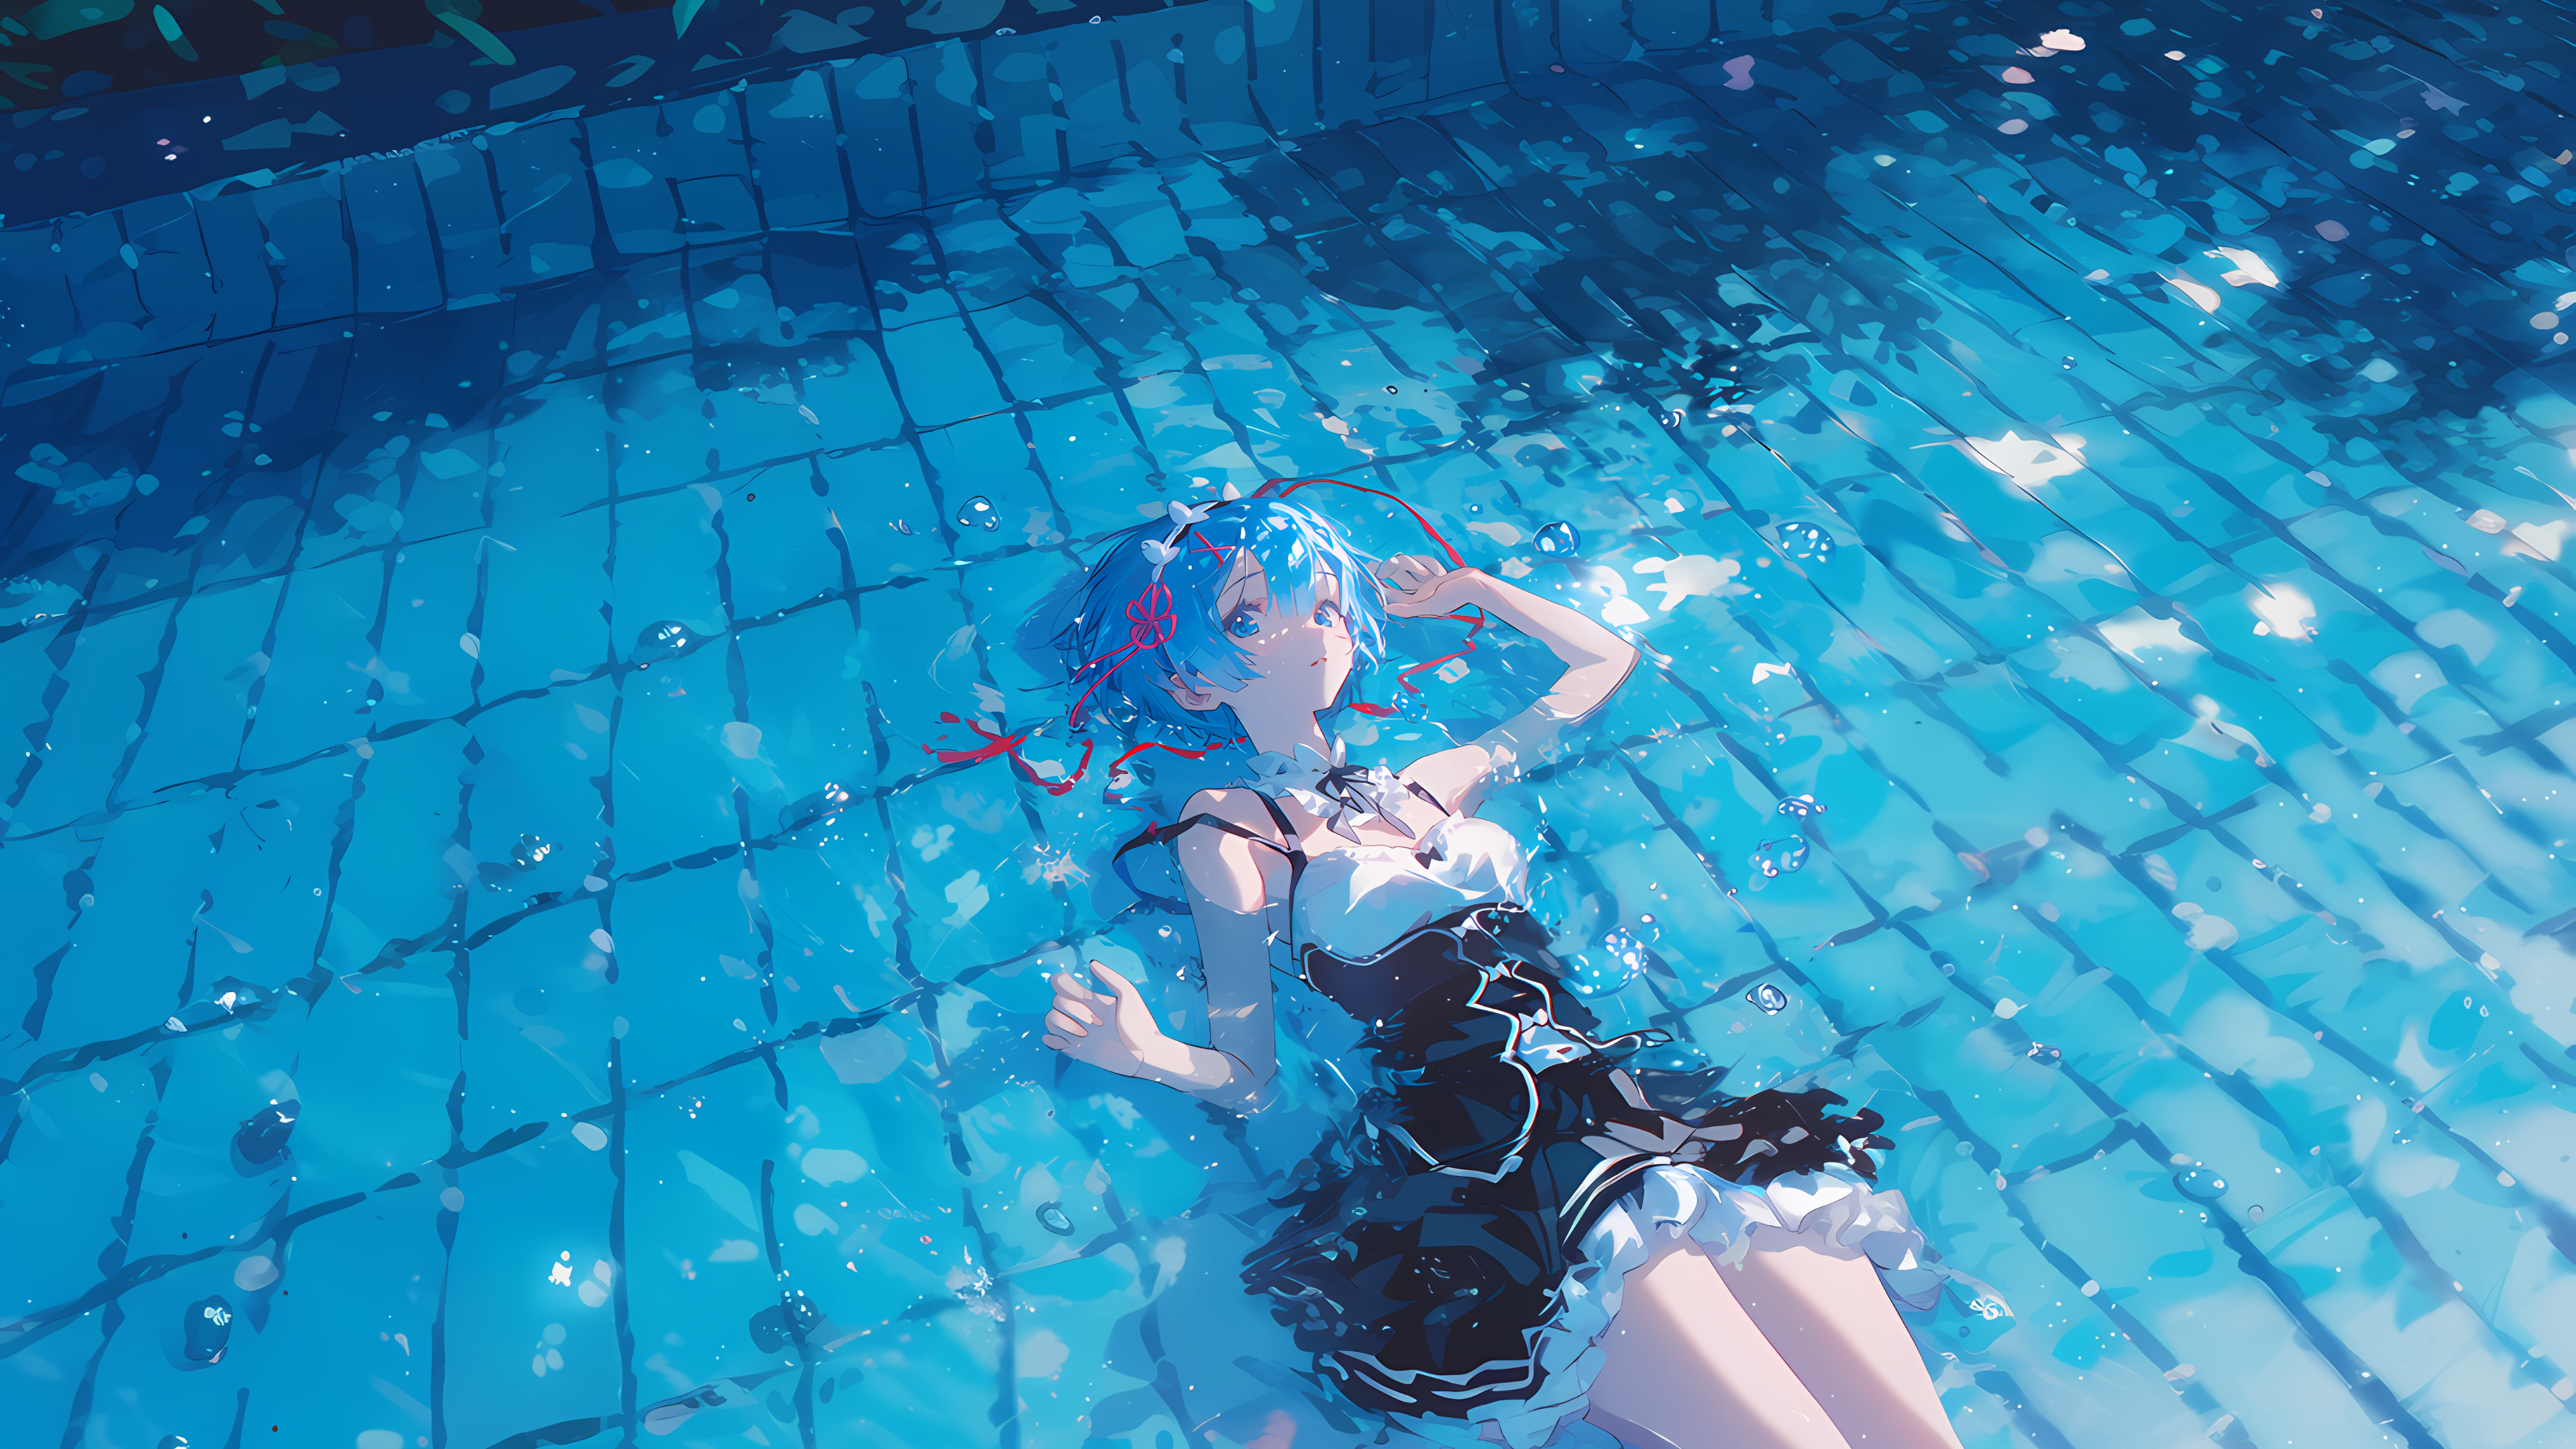
\includegraphics[width=16cm]{figure/封面.png} % ← 换成你的图片文件
			\end{minipage}
		};
	\end{tikzpicture}
\end{titlepage}